\documentclass{report}

\usepackage{hyperref}
\usepackage{color}
\usepackage[usenames]{xcolor}
\usepackage{tikz}

\usepackage{algorithm}
\usepackage{algpseudocode}

% New definitions
\algnewcommand\algorithmicswitch{\textbf{case}}
\algnewcommand\algorithmiccase{\textbf{}}
% New "environments"
\algdef{SE}[SWITCH]{Switch}{EndSwitch}[1]{\algorithmicswitch\ #1\ {\bf of}}{\algorithmicend\ \algorithmicswitch}%
\algdef{SE}[CASE]{Case}{EndCase}[1]{\algorithmiccase\ #1 :}{\algorithmicend\ \algorithmiccase}%
\algtext*{EndSwitch}%
\algtext*{EndCase}%

%\usepackage[T1]{fontenc}

\definecolor{lgray}{gray}{0.9}

\usepackage{listings}

\lstnewenvironment{tsllisting}[1]
{\vspace{3mm}
 \lstset{
    backgroundcolor=\color{lgray},
    basicstyle=\small\ttfamily, 
%    keywordstyle=\bfseries,
    keywordstyle=\underbar,
    identifierstyle=,
    commentstyle=\slshape,
    stringstyle=,
    showstringspaces=false,
    keywords={after,
              always,
              assert,
              assign,
              assume, 
              before,
              bool,
              case,
              choice, 
              cond,
              const,
              controllable, 
              default,
              derive,
              do, 
              else, 
              endtemplate,
              enum,
              export,
              false,
              forever, 
              fork, 
              function, 
              goal,
              if, 
              import,
              init,
              invisible, 
              mem,
              out,
              pause,
              break,
              post, 
              procedure, 
              process,
              return,
              sint,
              stop, 
              struct,
              task, 
              template, 
              true,
              typedef,
              uint,
              uncontrollable, 
              using, 
              void,
              while,
              wait},
    sensitive=false,
    morecomment=[l]{//},
    morecomment=[s]{/*}{*/},
    numberstyle=\tiny,
    stepnumber=1,
    numbersep=1pt,
    emphstyle=\bfseries,
    belowskip=0pt,
    aboveskip=0pt,
    #1
}}{\vspace{3mm}}

\lstnewenvironment{bnflisting}[1]
{\vspace{3mm}
 \lstset{
    backgroundcolor=\color{lgray},
    basicstyle=\small\ttfamily,
    keywordstyle=\underbar,
    identifierstyle=,
    commentstyle=\slshape,
    stringstyle=,
    showstringspaces=false,
    keywords=,
    sensitive=false,
    morecomment=[l]{//},
    morecomment=[s]{/*}{*/},
    numberstyle=\tiny,
    stepnumber=1,
    numbersep=1pt,
    emphstyle=\bfseries,
    belowskip=0pt,
    aboveskip=0pt,
    #1
}}{\vspace{3mm}}


\newcommand{\src}[1]{\texttt{#1}}

\newcommand{\tsl}{TSL2}

\newcommand{\comment}[1]{{\textit{\textbf{#1}}}}


\author{Leonid Ryzhyk}

\title{\tsl{} Reference Manual}

\begin{document}

\maketitle

\tableofcontents

\chapter{Introduction}

This document describes syntax and semantics of the Termite 
Specification Language, Version 2 (\tsl{}).  Information about the 
Termite synthesis tool can be found on the project website 
\url{http://termite2.org}.  See~\cite{Ryzhyk_WKLRSV_14} for a 
high-level overview of the project.

The rest of the manual consists of two parts.  
Chapter~\ref{s:overview} presents the main \tsl{} concepts and 
informally describes their semantics.  Chapter~\ref{s:reference} 
gives a more formal presentation of \tsl{} syntax.


\chapter{Overview}\label{s:overview}

\section{Static and dynamic namespaces}\label{s:o:namespace}

\tsl{} supports two namespaces: the \emph{static namespace} and 
the \emph{dynamic namespace}.  The static namespace is populated 
with compile-time objects: \emph{types} and \emph{constants}.  The 
dynamic namespace is populated with runtime objects: 
\emph{processes}, \emph{variables}, \emph{methods}, and 
\emph{wires}.  Static objects are uniquely identified by their 
name and syntactic scope.  In contrast, runtime objects can be 
instantiated multiple times within the specification and hence 
must be referred to relative to their runtime scope.  

\section{Templates}\label{s:o:templates}

Templates are the principal mechanism for managing both static and 
dynamic namespaces.  A template models a hardware of software 
entity, such as a device, an OS, or a device driver.  It declares 
a set of static objects (types and constants) and a set of runtime 
objects.  Static objects declared inside a template can be 
referenced from any part of the specification via the template 
name.  Runtime objects are instantiated together with the template 
and can be accessed via a reference to a template \emph{instance}.

The following template declares type \src{word} (static object) 
and variable \src{x} (runtime object):
\begin{tsllisting}{}
template A
  // type declaration
  typedef uint<16> word;
  // variable declaration
  export word x;
endtemplate
\end{tsllisting}
The \src{word} type is globally visible via the \src{::}-notation 
as \src{A::word}.  It can be used even if template \src{A} is 
never instantiated.  In contrast, variable \src{x} can only be 
accessed via an instance of \src{A}.  

Templates are instantiated inside other templates.  The sole 
exception is the \src{main} template, which is implicitly 
instantiated in the top-level scope.  Every complete \tsl{} 
specification must contain a template called \src{main}.  

In the following example, the \src{main} template creates an 
instance of \src{A}, making its variables accessible from 
\src{main} via instance name:
\begin{tsllisting}{}
template main
  instance A a;

  process pmain {
    // assigning variable x of template instance a.
    a.x = 16'd0;
  }
endtemplate
\end{tsllisting}

The template instantiation mechanism gives rise to an 
\emph{instance tree} with the \src{main} template at its root.  
Dynamic objects within the tree are accessed using hierarchical 
identifiers such as \src{a.x}.  This mechanism allows accessing 
objects down the branch of the instance tree, starting at the 
local template.  In practice, it is often necessary to access 
objects instantiated in other parts of the tree.  This is achieved 
in a structured way using \emph{template ports}.  

A template port is an alias to a template of a given type bound at 
the time of instantiation.  For example, template \src{B} below 
declares port \src{aa} of type \src{A}, which makes runtime 
objects in the scope of \src{A} visible from \src{B}.  Both 
templates are then instantiated in the \src{main} template, with 
the instance of \src{A} connected to port \src{aa} of \src{B}.
\begin{tsllisting}{}
// template B with port aa of type A
template B(A aa)
  process proc {
    aa.x = 16'd0;
  };
endtemplate

template main
  // create instances of A and B; connect port aa of
  // B to the instance of A.
  instance A a;
  instance B b(a);
endtemplate
\end{tsllisting}

The following diagram illustrates the resulting instance tree and 
the link between different branches of the tree via port \src{aa}.

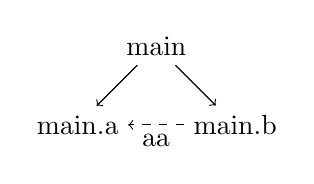
\begin{tikzpicture}
    \node[rectangle] (m) at (0,1) {main};
    \node[rectangle] (a) at (-1,0) {main.a};
    \node[rectangle] (b) at (1,0) {main.b};
    \path[->] (m) edge (a);
    \path[->] (m) edge (b);
    \path[->,dashed] (b) edge node[auto]{aa} (a);
\end{tikzpicture}

Another mechanism for managing name spaces is \emph{template 
inheritance}.  Using inheritance, one can create generic templates 
that capture common properties of a family of entities, leaving 
some of the properties underspecified.  The generic template can 
be specialised by a child template that fills in the missing 
details.  For example, the following template models common 
device-class callbacks that must be implemented by any OS 
specification for the IDE device class.  Note that callbacks are 
defined without bodies, as the exact behaviour is OS-specific.
\begin{tsllisting}{}
template ide_os
  procedure void write_sectors(uint<48> lba, 
    uint<16> sectors, uint<32> buf, bool xfer_error);
  procedure void read_sectors(uint<48> lba, 
    uint<16> sectors, uint<32> buf, bool xfer_error);
  procedure void reset();
  ...
endtemplate
\end{tsllisting}
This template is specialised by the \src{l4\_ide\_os} template,
that describes the IDE driver interface defined by the seL4 OS.
\begin{tsllisting}{}
template l4_ide_os(l4_ide_drv drv)
  // the derive statement is used to establish the 
  // inheritance relation
  derive ide_os;

  // additional specification items can be declared in the 
  // child template
  export iostatus reset_status = ionone;

  // the child template implements methods inherited from 
  // the parent.
  procedure void write_sectors(uint<48> lba, 
    uint<16> sectors, uint<32> buf, bool xfer_error)
  {
    assert (lba == r_lba);
    ...
  }
\end{tsllisting}

A template that is missing a method body or a wire assignment 
(Section~\ref{s:o:variables}) is called \emph{pure template}.  
Pure templates can be used in derive statements and in port 
declarations, however they cannot be instantiated.

Template inheritance is subject to the following rules:
\begin{itemize}
    \item Derived template must re-declare all ports of all its 
        parent templates with the same names and types.  It can 
        also declare additional ports not found in any of its 
        parents.

    \item If a template has multiple parent templates, then the 
        namespaces of parent templates (consisting of variable, 
        wire, method, goal, and process names) must not overlap.

    \item If the derived template re-declares a wire or method 
        declared in one of its parents, the new declaration must 
        have the same signature as the parent declaration.

    \item The child template can override wire and method 
        declarations of its parent templates.  Other parts of the 
        parent template, including variable, goal, and process 
        declarations, are inherited by the child template and 
        cannot be overriden.
\end{itemize}



\section{Execution model}\label{s:o:execmodel}

All state transitions in \tsl{} occur in the context of 
\emph{processes}.  Multiple processes can be enabled at the same 
time; however exactly one process participates in each individual 
transition.  Process transitions are atomic with respect to other 
processes.  Process that performs the next transition is chosen by 
the scheduler among enabled processes.  Scheduling is fair, i.e., 
if a process stays enabled sufficiently long, it will eventually 
get scheduled.

Processes are declared inside templates using the \src{process} 
keyword.  Such processes become runnable in the initial state of 
the system.  Additional processes can be spawned at runtime using 
the \src{fork} construct.  \tsl does not allow recursion, hence 
only a bounded number of processes can be spawned at any time.  

In the following example, template \src{A} contains a single 
static process \src{psndrcv}, which spawns two subprocesses 
\src{psend} and \src{preceive}.
\begin{tsllisting}{}
template A

process psndrcv {
  fork {
    psend:    forever send();
    preceive: forever receive();
  };
  shutdown();
};
...

endtemplate
\end{tsllisting}

%In addition to statically and dynamically created processes, every 
%\tsl specification contains an implicit \emph{idle} 

A process state transition starts in the current program location 
and stops at the next \emph{pause location}.  Pause locations can 
be explicit or implicit.  Explicit pause locations are created 
using \src{pause}, \src{wait}, and \src{stop} constructs.  
Implicit pause locations are introduced automatically by the 
compiler in the following cases:

\begin{itemize}
    \item Before \src{fork} statements
    \item Before magic blocks~\ref{s:o:magic}
    \item On exit from controllable tasks (see below)
\end{itemize}

A process can invoke \emph{methods} declared inside its own 
template as well as in other template instances, via hierarchical 
identifiers discussed in the previous section.  There are three 
types of methods in \tsl{}: \emph{functions}, \emph{procedures}, 
and \emph{tasks}.  Functions and procedures must complete 
instantaneously, i.e., they are not allowed to contain explicit or 
implicit pauses.  In addition, functions are not allowed to have 
side effects, i.e., they cannot modify any global variables, 
perform pointer dereferences, or contain assertions (pointer 
dereferences and assertions statements can have the side effect of 
taking the system into an error state).  

Tasks can consist of multiple atomic transitions.  A task can have 
an optional \src{controllable} or \src{uncontrollable} qualifier.  
Controllable tasks are the only kind of task that can be invoked 
from synthesised code; although they can also be called from 
manually written code.  They are used to model the device register 
interface and OS callbacks.  In the current implementation of the 
\tsl{} compiler, controllable tasks are subject to additional 
constraint: they are not allowed to contain internal pause 
locations, i.e., a controllable task must always complete in a 
single transition. 

Uncontrollable tasks represent driver methods invoked by the OS or 
the device.  Uncontrollable tasks are the only kind of task that 
can contain automatically generated code, i.e., a magic block can 
only be placed inside an uncontrollable task.  

Controllable task invocations introduce implicit pause locations 
on return from the task.  In the following example execution of 
process \src{p1} that invokes controllable task \src{t1} consists 
of two transitions.
\begin{tsllisting}{}
template A
  uint<16> x;
  uint<16> y;

  process p1 {
    x = t1();
    y = x
  };

  task uncontrollable void t1(uint<16> arg) {};
endtemplate
\end{tsllisting}
The first transition controllable task \src{t1} and stores its 
retusr value in variable \src{x}.  An implicit pause is inserted 
at the task return location.  The remainder of the process is 
executed in the second transition.  Note that other processes can 
run and potentially modify the value of \src{x} in between 
transitions 1 and 2.

Tasks without \src{controllable} and \src{uncontrollable} 
qualifiers behave as if the body of the task was inlined at the 
call location.  No additional pauses are inserted before or after 
the task.

\section{Variables and wires}\label{s:o:variables}

\emph{Variables} are used to store state that persists for the 
lifetime of the variable.  Variables in \tsl{} can be declared in 
the template, process, or method scope.  Template-scope variables, 
also called \emph{global variables}, are instantiated together 
with the template and are visible from anywhere inside the 
template.  In addition, variables declared with the \src{export} 
qualifier can be accessed from other templates via their 
hierarchical identifiers.  Process and method variables are only 
visible within the syntactic scope of the process or method where 
they are declared.

In contrast to variables, \emph{wires} are simply aliases to 
expressions defined over global variables and are not allocated 
their own storage.  Wires keep their values throughout a 
transition and are updated at the end of the transition.  Initial 
value of a wire is computed based on initial values of global 
variables.

\begin{tsllisting}{}
template A
  uint<16> x = 0;
  wire uint<16> w = x + 1;
endtemplate
\end{tsllisting}


\section{Correctness specifications}\label{s:o:correctness}

\tsl{} provides two mechanisms for specifying correctness 
conditions on system behaviour:
\begin{itemize}
    \item \emph{Goals.} A goal is a side-effect-free boolean 
        expression over global variables that must hold infinitely 
        often in any infinite run of the system.  A template can 
        declare any number of goals.  In addition, \tsl{} defines
        an implicit goal, which requires the system to be outside 
        of a magic block infinitely often; in other words, the 
        system cannot stay inside a magic block forever.
    \item \emph{Assertions.}  An \src{assert} statement can be 
        placed anywhere inside processes, tasks, and procedures.  
        It defines a condition whose violation immediately 
        transitions the system to an error state.
\end{itemize}

The following example illustrates the use of goals and assertions in the 
IDE OS template:

\begin{tsllisting}{}
template l4_ide_os(ide_drv drv, ide_dev dev)

// The driver/OS interface must infinitely often be in 
// a state with no outstanding I/O requests.
goal drv_goal = (req_status == ionone);

task controllable void cache_ack(){
    assert ((req_status == iosuccess_cache) || 
            (req_status == ioerror_cache));
    req_status = ionone;
};
endtemplate
\end{tsllisting}

\section{Magic blocks}\label{s:o:magic}

A \emph{magic block} is a place holder for automatically generated 
code.  Given a \tsl{} specification with one or more magic block,
Termite aims to replace magic blocks with executable code so that 
the resulting complete system satisfies all its goals and does not 
violate any assertions.

%Note that for synthesis to succeed the resulting system must 
%satisfy all correctness conditions described in the following 
%section, and not just magic block postconditions.

\begin{tsllisting}{}
template main
  task uncontrollable bool probe() {
    // Magic block
    ...;
    assert ((os.reset_status == iosuccess) ||
            (os.reset_status == ioerror));
    if (os.reset_status == iosuccess) {
      return true;
    } else {
      return false;
    };
};
endtemplate
\end{tsllisting}

%The second type of magic blocks are magic blocks with 
%\emph{goals}.  These are needed because not all correctness 
%conditions can be captured using postconditions and assertions.  
%For correctness conditions specified using goals (see 
%Section~\ref{s:o:correctness}), the synthesis algorithm computes a 
%strategy for each goal; however the scheduling of strategies is 
%left to the user, i.e., the user decides when to execute each 
%strategy by assigning goals to magic blocks. \comment{TODO: I 
%still have not figured out the exact meaning of this construct.}

%\section{Constraints on the environment}

\chapter{Syntax reference}\label{s:reference}

\section{Literals}\label{s:r:literals}

\tsl{} supports boolean literals ``\src{true}'' and 
``\src{false}'' and Verilog-style binary, octal, decimal and 
hexadecimal integer literals.  The exact number of bits can be 
specified for each integer literal.  

\begin{bnflisting}{}
<intLit> := <decNumber>
          | [<width>] "'b"  <binNumber>
          | [<width>] "'sb" <binNumber>
          | [<width>] "'o"  <octNumber>
          | [<width>] "'so" <octNumber>
          | [<width>] "'d"  <decNumber>
          | [<width>] "'sd" <signedDecNumber>
          | [<width>] "'h"  <hexNumber>
          | [<width>] "'sh" <hexNumber>
<width> := <decNumber>
\end{bnflisting}

Examples of integer literals:
\begin{tsllisting}{}
uint<8> x;
sint<8> y;

x = 255;
x = 8'd35;
x = 8'b01010101;
x = 8'b1;

y = 8'sb11111111;
y = 8'sd-6;
\end{tsllisting}

In case literal width is not specified explicitly, the compiler 
assumes the smallest width sufficient to encode the given integer 
value, for example literal $5$ is assumed to be $3$ bits wide, as 
$3$ bits are sufficient to encode values between $0$ and $5$.  The 
compiler does not perform automatic truncation or extension of 
integers.  For example, the following assignment statement is 
invalid, as the left and the right-hand sides of assignment have 
different width:

\begin{tsllisting}{}
uint<8> x = 0; // error: x has width 8, while
               // literal 0 has width 1

uint<8> y = 8'd0; // ok
\end{tsllisting}


\section{Identifiers}\label{s:r:identifiers}

Identifiers are used to refer to static and runtime objects 
(Section~\ref{s:o:namespace}).  \tsl{} supports three forms of 
identifiers: \emph{simple identifiers}, \emph{statically scoped 
identifiers}, and \emph{hierarchical identifiers}.

\paragraph{Simple identifiers.}  A simple identifier is a name of 
a static or runtime object visible within the current syntactic 
scope.  This includes objects declared within the current scope or 
in one of its parent scopes.  For example, simple identifier 
\src{x} used in a method body can refer to a local variable or 
argument of the method, template-global variable, or a type or 
constant declared in the template or top-level scope.

\begin{bnflisting}{}
<ident> := (<letter> | "_") (<letter> | <digit> | "_")*
\end{bnflisting}

\paragraph{Statically scoped identifiers.} These identifiers refer 
to static objects declared within template scope.  They can be 
used to refer to static objects declared in templates other than 
the local template.

\begin{bnflisting}{}
<staticIdent> := <ident> "::" <ident>
\end{bnflisting}
where the first identifier is a template name.

\paragraph{Hierarchical identifiers.}  These identifiers are used 
to refer to runtime objects outside of the current syntactic 
scope.  A hierarchical identifier is a dot-separated sequence of 
literals that traverses the instance tree 
(Section~\ref{s:o:templates}) via port and instance names:

\begin{bnflisting}{}
<hierarchicalIdent> := <ident> ["." <ident>]*
\end{bnflisting}

The following example illustrates the use of different types of 
identifiers.

\begin{tsllisting}{}
template A
  typedef uint<16> word;
  export word x;
endtemplate
    
template B(A aa)
  // Reference to the word type declared in template A
  // via static scoped identifier;
  A::word y;

  process proc {
    // In the following statement:
    // * y is a simple identifier that refers to a variable
    //   declared in the local template
    // * aa.x is a hierarchical identifier that refers to
    //   variable x declared in an instance of template A
    //   referred to by the aa port of template B.
    y = aa.x;
  };
endtemplate

template main
  // create instances of A and B; connect port aa of
  // B to the instance of A.
  instance A a;
  instance B b(a);
endtemplate
\end{tsllisting}


\section{Types}

Type expressions can occur in various contexts in a \tsl{}
specification, including variable, method, wire, type, and 
constant declarations.  The language currently supports arbitrary 
fixed-width signed and unsigned integers, booleans, enums, 
structs, arrays, and pointers.

\begin{bnflisting}{}
<typeSpec>   := ( <sintType>    // signed int
                | <uintType>    // unsigned int
                | <boolType>    // boolean
                | <userType>    // user-defined type name
                | <enumType>    // enumeration
                | <structType>) // struct
                <typeModifier>* // type modifiers

<sintType>   := "sint" "<" <decimalNumber> ">"
<uintType>   := "uint" "<" <decimalNumber> ">"
<boolType>   := "bool"
<userType>   := <staticIdent>
<enumType>   := "enum" "{" (<ident> ",")*  <ident> "}"
<structType> := "struct" "{" (<typeSpec> <ident> ";")+ "}"

// A type modifier is either array dimension or the pointer
// modifier ("*")
<typeModifier> := ("[" <expr> "]")
                | "*"
\end{bnflisting}

\tsl{} enum's are different from C-style enum's in that they are 
not integers.  In particular, a variable of enum type cannot be 
cast to an integer.  Such a variable can only take one of the 
values in the enumeration and not any other arbitrary integer 
value.  Furthermore, an enum declaration cannot assign integer 
values to enumerators.

Type expressions are subject to the following constraints:
\begin{itemize}
    \item Enumerations can only be declared in \src{typedef}
        statements, i.e., they cannot be declared inline in 
        variable or method declarations.  This ensure that every 
        enum type has a name.
    \item Variable-size arrays are not supported: array dimensions 
        must be compile-time constants.
\end{itemize}

Examples of type expressions:

\begin{tsllisting}{}
typedef uint<16> t1;
typedef sint<13> t2;
typedef enum {e1, e2, e3} t3;
typedef struct {t1 f1; t2 f2;} t4;
const t1 c1 = 16'd5;
typedef t4[c1] arrtype;
typedef struct {bool f1; uint<16>[10] f2;} * structptr;
\end{tsllisting}

\section{Expressions}

\tsl{} expressions are constructed from identifiers 
(Section~\ref{s:r:identifiers}), literals
(Section~\ref{s:r:literals}), and method 
invocations~\ref{s:r:invocation} using operators summarised in 
Table~\ref{t:ops} in the order of decreasing precedence.

\begin{table}
\begin{small}
\noindent
\begin{tabular}{|l|l|l|l|p{0.3\linewidth}|}
    \hline
    {\bf operator}                   & {\bf syntax} & {\bf arg type} & {\bf res type} & {\bf comment} \\
    \hline
    \hline 
    {\tt[:]}                         & {\tt e[l:h]} & integer        & unsigned int   & bit slice \\
    {\tt[~]}                         & {\tt e[i]}   & array          & -              & array index \\
    {\tt.}                           & {\tt e.f}    & struct         & -              & struct field \\
    {\tt\verb=->=}                   & {\tt\verb=e->f=}  & struct pointer & -              & struct dereference \\
    \hline
    \src{!}                          & prefix  & bool           & bool           & boolean negation \\
    {\tt\verb=~=}                    & prefix  & integer        & integer        & bit-wise negation \\
    {\tt-}                           & prefix  & integer        & integer        & unary minus \\
    {\tt*}                           & prefix  & pointer        & -              & pointer dereference \\
    {\tt \&}                         & prefix  & any            & pointer        & address-of \\
    \hline
    {\tt ==, !=}                     & infix   & any            & bool           & \\
    {\tt\verb#<, <=, >, >=#}         & infix   & integer        & bool           & \\
    \hline    
    {\tt\&}                          & infix   & integer        & integer        & bit-wise and \\
    \hline    
    {\tt |}                          & infix   & integer        & integer        & bit-wise or \\
    \hline    
    {\tt\verb#^#}                    & infix   & integer        & integer        & bit-wise xor \\
    \hline    
    {\tt ++}                         & infix   & integer        & integer        & bit-vector concatenation \\
    \hline    
    {\tt\&\&}                        & infix   & bool           & bool           & boolean and \\
    \hline    
    {\tt||}                          & infix   & bool           & bool           & boolean or \\
    \hline    
    {\tt\verb#=>#}                   & infix   & bool           & bool           & boolean implication\\
    \hline    
    {\tt*}                           & infix   & integer        & integer        & multiplication \\
    \hline    
    {\tt\%}                          & infix   & integer        & integer        & residue \\
    \hline    
    {\tt+}                           & infix   & integer        & integer        & plus \\
    \hline    
    {\tt-}                           & infix   & integer        & integer        & minus \\
    \hline
\end{tabular}
\end{small}
\caption{\tsl{} operators}\label{t:ops}
\end{table}

In addition, \tsl{} supports three kinds of conditional 
expressions: \src{if-else} expressions (or ternary expressions), 
\src{case}-expressions, and \src{cond}-expressions.  

\begin{bnflisting}{}
<ternExp> := "if" <expr> <expr> "else" <expr>
<caseExp> := "case" "(" <expr> ")" "{" (<expr> ":" <expr> ";")* 
                 (<expr> ":" <expr> ";")* 
                 ["default" ":" <expr> ";"]
            "}"
<condExp> := "cond" "{"
                  (<expr>    ":" <expr> ";")*
                  ["default" ":" <expr> ";"]
              "}"
\end{bnflisting}

A \src{case}-expression chooses a value based on the value of its 
key expression, whereas a \src{cond}-expression chooses a value to 
return by evaluating a series of conditions in order.  Note that 
\src{if-else} expressions are different from \src{if} statements 
described in Section~\ref{s:r:coniditional}.

Finally, \tsl{} supports struct expressions with explicit or 
implicit field names:

\begin{bnflisting}{}
<structExp>   := <staticIdent> "{" 
                     (<namedFields> | <anonFields>) 
                 "}"
<namedFields> := "." <ident> "=" <expr> 
                 [("," "." <ident> "=" <expr>)*]
<anonFields> := <expr> 
                 [("," <expr>)*]
\end{bnflisting}

Note that \tsl{} does not provide type casting operations.  In 
particular, it is impossible to convert a pointer to an integer or 
an integer to a pointer.  In addition, the \tsl{} compiler 
enforces the following type and memory safety rules:
\begin{itemize}
    \item No arithmetic operations are allowed on pointers or enum's
    \item Bit-wise operators must be applied to integer operands 
        of the same width
    \item \src{==} and \src{!=} operations can only be applied to 
        operators of identical types (including width and 
        signedness)
    \item Labels in a \src{case}-expression and conditions in a 
        \src{cond}-expression must be side-effect free
    \item All branches of a \src{case}, \src{cond}, or \src{if-else}
        expression must return values of the same type
    \item Lower and upper bounds of a bit slice must be constant 
        expressions, lower bound must be less than or equal to the 
        upper bound, and both bounds must be smaller than the width
        of the argument.
    \item The address-of operator (\src{\&}) can only be applied 
        to memory variables (see Section~\ref{s:r:localvar}).
\end{itemize}

\subsection{Non-deterministic expressions}

Special expression \src{*} is used to generate non-deterministic 
values of arbitrary type.  The exact type is derived from the 
context, as illustrated in this example:
\begin{tsllisting}{}
x = *;  // Generate random value of the same type as x.
f(*,*); // Generate random values that match argument 
        // types of f.
\end{tsllisting}
Note that \src{*} cannot be used as an atom in a complex expression,
for example, the following is not valid:
\begin{tsllisting}{}
x = * + 2; // Invalid use of *
\end{tsllisting}

\subsection{L-expressions}\label{s:r:lexpr}

\emph{L-expressions} are a subset of \tsl{} expressions that can 
be used as the left-hand side of assignment statements and as 
output arguments of methods.  L-expressions are defined by the 
following rules:
\begin{enumerate}
    \item Names of variables visible in the current scope, 
        including global variables, local variables, and function 
        arguments are L-expressions
    \item All valid expressions of the form \src{*e} and 
        \src{e->f} are L-expressions.
    \item If \src{e} is an L-expression then the following are 
        also L-expressions:
        \begin{itemize}
            \item \src{e.f}
            \item \src{e[i]}
            \item \src{e[l:h]}
        \end{itemize}
\end{enumerate}

\subsection{Expression evaluation}

Expression evaluation order matters in cases when expression 
operands contain method calls, which may have side effects.  
All expression operands are evaluated before the expression itself is evaluated.  In 
particular, if the expression contains method calls, then all of 
these calls are performed before the expression is evaluated.
\comment{This description reflects how the compiler works 
at the moment; however this behaviour is counter-intuitive and 
should be fixed to be more C-like}.

\section{Statements}

Statements are used to define process behaviour and occur in 
process and method bodies and prefix-blocks 
(Section~\ref{s:r:always}).

\begin{bnflisting}{}
<statement> := <varDecl>  // local var declaration
             | <sseq>     // sequential block
             | <spar>     // parallel blocks
             | <sforever> // forever loop
             | <sdo>      // do loop
             | <swhile>   // while loop
             | <sfor>     // for loop
             | <sbreak>   // break out of a loop
             | <schoice>  // nondeterministic choice
             | <spause>   // pause
             | <swait>    // wait on a condition
             | <sstop>    // stop
             | <sassert>  // assertion
             | <sassume>  // assumption
             | <site>     // if-then-else statement
             | <scase>    // case statement
             | <sinvoke>  // method invocation
             | <sassign>  // variable assignment
             | <sreturn>  // return statement
             | <smagic>   // magic block
\end{bnflisting}

\subsection{Variable declarations}\label{s:r:localvar}

Variable declaration statements are used to declare local 
variables visible within the syntactic scope of a process, method 
or prefix-block.  A local variable is visible everywhere within 
its scope regardless of the exact location where it has been 
declared.  A variable declaration consists of an optional 
\src{mem} qualifier, variable type and name and optional initial 
assignment:
\begin{bnflisting}{}
<varDecl> := ["mem"] <typeSpec> <ident> ["=" <expr>]
\end{bnflisting}
The \src{mem} qualifier labels the variable as in-memory variable,
which allows the address-of operator to be applied to this 
variable or any of its fields.  In addition, in performing pointer 
analysis of a \tsl{} specification, one can assume that a pointer 
can only point to an in-memory variable of a matching type.

In case variable declaration does not specify an initial value for 
the variable, the value for the variable is chosen 
non-deterministically.

\subsection{Sequential blocks} 

C-style sequential blocks:
\begin{bnflisting}{}
<sseq> = "{" (<statement> ";")* "}"
\end{bnflisting}

\subsection{Parallel blocks}\label{s:r:fork}

The \src{fork} construct is used to spawn several child processes.  
\begin{bnflisting}{}
<spar> := "fork" "{" 
               (<ident> ":" <statement> ";")*
          "}"
\end{bnflisting}
Each child process is assigned a unique label, which helps 
identify processes during debugging.  The spawning process blocks 
waiting for all forked processes to terminate.  Forked processes 
terminate when all of them have reached a \emph{final} state 
(i.e., a process cannot terminate without waiting for its siblings 
to be in final states as well).  A process is in a final state 
when it reaches either the end of its execution (i.e., executes 
its last instruction) or a \src{stop} statement 
(Section~\ref{s:r:pause}).  

In the following example two dynamically spawned processes send 
and receive data in an infinite loop.
\begin{tsllisting}{}
process psndrcv {
  fork {
    psend:    forever {
                  stop;   // final state
                  send();
              };
    preceive: forever {
                  stop;   // final state
                  receive();
              };
  };
  shutdown();
};
\end{tsllisting}
At each iteration of the loop, they go through final states marked 
by the \src{stop} statements.  When both processes are in their 
respective final states, the entire \src{fork} block \emph{may} 
terminate, with the parent process moving on to the next 
statement; however, it is not required to terminate and can 
continue executing \src{forever} loops.  The choice between 
terminating and continuing execution is performed 
nondeterministically by the environment.  In contrast, in the 
following example, once both processes reach their final control 
locations, the fork block terminates instantaneously, as neither 
process can execute any more transitions:
\begin{tsllisting}{}
process psndrcv {
  fork {
    psend:    send();
    preceive: receive();
  };
  shutdown();
};
\end{tsllisting}

\subsection{Loops}  

In addition to conventional do, while, and for loops, \tsl{}
supports forever loops, which are equivalent to \src{while(true)}.
\begin{bnflisting}{}
<sdo>      := "do" <statement> "while" "(" <expr> ")"
<swhile>   := "while" "(" <expr> ")" <statement>
<sfor>     := "for" "(" [<statement>] ";" 
                        <expr> ";" 
                        <statement> ")" 
                  <statement>
<sforever> := "forever" <statement>
\end{bnflisting}

At the moment \tsl{} does not allow \emph{instantaneous loops}, 
i.e., every possible path through the loop body must contain an 
explicit or implicit pause location (Section~\ref{s:o:execmodel}).  
This restriction is enforced by the compiler via a simple static 
check.  Note that there is no implicit pause before the body of 
the loop, i.e., execution enters the loop instantaneously and 
continues until reaching a pause location inside the loop.  For 
example, in the following example, process \src{foo} executes two 
transitions: (1) \src{x=16'd0; (x<1) == true; x=x+16'd1}, and (2) 
\src{(x<1) == false; y=16'd0}.
\begin{tsllisting}{}
process foo {
    x = 16'd0;
    while (x < 1) {
        x = x + 16'd1;
        pause;
    };
    y = 16'd0;
};
\end{tsllisting}

The \src{break} statement can be used anywhere inside a loop to 
transfer control to the first instruction following the body of 
the innermost loop.

\subsection{Non-deterministic choice}  The \src{choice} construct 
allows the environment to non-deterministically choose between
two or more actions:
\begin{bnflisting}{}
<schoice> := "choice" "{"
               (<statement> ";")*
             "}"
\end{bnflisting}

\subsection{Pause statements}\label{s:r:pause}

\tsl{} offers three ways to insert an explicit pause location 
(Section~\ref{s:o:execmodel}) in the control flow of a process or 
method: \src{wait}, \src{pause}, and \src{stop}
statements.
\begin{bnflisting}{}
<swait>  := "wait" "(" <expr> ")"
<spause> := "pause"
<sstop>  := "stop"
\end{bnflisting}

The \src{wait} statement inserts a pause location and disables the 
current process until the wait condition becomes true.  If the 
wait condition stays true for sufficiently long time, the process 
is guaranteed to eventually leave the pause location.  Note that 
if the wait condition is already true when the process enters the 
pause location, the current transition terminates anyway.

The \src{pause} statement is a shortcut for \src{wait(true)}.  
\src{stop} behaves like \src{pause}, but additionally marks the 
current process state as final (Section~\ref{s:r:fork}).

\subsection{Assertions} 

An assertion behaves as a no-op if its argument evaluates to true, 
and causes a transition to an error state otherwise.
\begin{bnflisting}{}
<sassert> := "assert" "(" <expr> ")"
\end{bnflisting}
The argument of an \src{assert} statement must be a 
side-effect-free expression.

\subsection{Assumptions}  

\begin{bnflisting}{}
<sassume> := "assume" "(" <expr> ")"
\end{bnflisting}

Assumptions are used to constrain possible system behaviours.  
Similar to assertions, they specify constraints that must hold for 
any valid execution of the system.  However, while an assertion 
causes transition to an error state if its condition is violated, 
the \src{assume} statement prunes all transitions that violate the 
assumption.

Assumptions are particularly useful in imposing restrictions on 
randomly generated values, as illustrated by the following 
example.
\begin{tsllisting}{}
// assign random values for stopbits and data vars
stopbits  = *;
data      = *;
// only certain combinations of stopbits and data values 
// are valid
assume(((stopbits==UART_STOP_BITS_15) && (data==4'd5)) || 
        ((stopbits==UART_STOP_BITS_2) && (data!=4'd5)));
case (data) {
    4'd5:       data_bits = CUART_DATA5;
    4'd6:       data_bits = CUART_DATA6;
    4'd7:       data_bits = CUART_DATA7;
    4'd8:       data_bits = CUART_DATA8;
    default: assume(false); // other values are not allowed
};
\end{tsllisting}

\subsection{Conditional statements}\label{s:r:coniditional}

\tsl{} supports C-style \src{if-else} statements and \src{case} 
statements:
\begin{bnflisting}{}
<site>  := "if" "(" <expr> ")" <statement>
             ["else" <statement>]
<scase> := "case" "(" <expr> ")" "{"
             (<expr> ":" <statement> ";")*
             ["default" ":" <statement> ";"
           "}"
\end{bnflisting}

Labels of the \src{case} statement can be arbitrary 
side-effect-free deterministic expressions of a matching type.  At 
runtime, the first matching label is selected.  At most one branch 
of a case statement is executed; execution does not fall through 
to the next label automatically.  Unlike in C, the \src{break} 
statement cannot be used to break out of a case clause.  While 
\src{break} is allowed inside the body of a \src{case}, it has the 
effect of breaking out of the innermost loop.

\subsection{Method invocation}\label{s:r:invocation}

Method invocations can occur as atoms in expressions as well as 
standalone statements.  Method name is a hierarchical identifier 
that refers either to a method declared in the local template or 
exported from another template.
\begin{bnflisting}{}
<sinvoke> := <hierarchicalIdent> "(" [<expr> [("," <expr>)*]] ")"
\end{bnflisting}
Method arguments must match the number and types of formal 
arguments in the method declaration.  Output 
arguments~\ref{s:r:method} must be L-expressions~\ref{s:r:lexpr}.

\subsection{Assignment statements}

\begin{bnflisting}{}
<sassign> := <expr> "=" <expr>
\end{bnflisting}

The left-hand side of an assignment statement must be an 
L-expression (Section~\ref{s:r:lexpr}).  Types of left- 
and right-hand side expressions must match, including sign 
and width for integer types.

\subsection{Return statements}\label{s:r:return}

\begin{bnflisting}{}
<sreturn> := "return" [<expr>]
\end{bnflisting}

Return statements are only allowed in method bodies.  If the 
method is a \src{void} method, return must not have an argument; 
otherwise it must have an argument whose type matches the return 
type of the method.  Every path through a non-void method must 
contain a \src{return} statement.  Statements following a 
\src{return} statement are ignored and control transfers to the 
location immediately following the call site.  

If the method is a controllable task then an implicit pause 
(Section~\ref{s:o:execmodel}) is introduced at the return 
location.  

%In this case, if the value returned by the task is used as the 
%right-hand side of an assignment, the value of the left-hand side 
%is modified at the beginning of the next transition performed by 
%the process.

\subsection{Magic blocks}

\begin{bnflisting}{}
<smagic> := "..."
\end{bnflisting}

See section~\ref{s:o:magic}.

\section{\tsl{} file structure}

A \tsl{} file consists of \emph{import} statements, type 
declarations, constant declarations, and template declarations.

\begin{bnflisting}{}
<tslFile>  := <specItem>*
<specItem> := <import>
           |  <typeDecl>
           |  <const>
           |  <template>
\end{bnflisting}

\section{Import statements}

Import statements are used to combine multiple \tsl{} files.  They 
are only allowed in the top-level syntactic scope, i.e., they are 
illegal inside template of type declarations.  An import statement 
consists of the \src{import} keyword followed by file path in 
angle brackets:
\begin{tsllisting}{}
import<ide_dev.tsl>
import<os/ide_tsl2/l4_ide.tsl>
import<../../os/ide_tsl2/ide_class.tsl>
\end{tsllisting}
The \tsl{} compiler appends this path to the current directory and 
to each import directory, specified via the \src{-I} command line 
switch, in order, until a  file with this name is found.

\section{Type declarations}\label{s:r:typedecl}

Type declarations can be placed in the top-level scope or in a
template scope.

\begin{bnflisting}{}
<typeDecl> := "typedef" <typeSpec> <ident>
\end{bnflisting}

\section{Constant declarations}\label{s:r:constant}

Constant declarations can be placed in the top-level scope or in a
template scope.  The value of a constant is an expression that can
be evaluated at compile time.

\begin{bnflisting}{}
<const> := "const" <typeSpec> <ident> "=" <expr>
\end{bnflisting}

Examples:

\begin{tsllisting}{}
typedef struct {bool f1; uint<16> f2;} stype;

const bool     b = true;
const uint<16> u = 16'd5;
const stype    s = stype {.f1 = b, .f2 = u};
\end{tsllisting}


\section{Templates}

Templates must be declared within the top-level scope, i.e., 
nested template declarations are not allowed.  Template 
declaration has the following syntax:
\begin{bnflisting}{}
<template> := "template" <ident> [(<portDeclarations>)]
                  (<templateItem> ";")*
              "endtemplate"
\end{bnflisting}
Here, \src{<portDeclarations>} is a comma-separated list of port 
declarations, described in Section~\ref{s:o:templates}.  A 
template item is one of:
\begin{itemize}
    \item Derive statement
    \item Instance declaration
    \item Type declaration
    \item Constant declaration
    \item Global variable declaration
    \item Init block
    \item Prefix block
    \item Process
    \item Method
    \item Goal
    \item Wire declaration
\end{itemize}

Derive statements and instance declarations were considered in 
Section~\ref{s:o:templates}.  Type declarations and constant 
declarations were considered in Sections~\ref{s:r:typedecl} and
\ref{s:r:constant}.  We describe the remaining kinds of template 
items below.

\subsection{Global variable declarations}

Global variables (Section~\ref{s:o:variables}) are declared in the 
template scope.  The declaration syntax is the same as for local 
variables (Section~\ref{s:r:localvar}) with the optional 
\src{export} qualifier, which indicates that the variable can be 
accessed from outside the template:

\begin{bnflisting}{}
<gvarDecl> := ["export"] <varDecl>
\end{bnflisting}

Similar to local variable declarations, if the declaration does 
not specify an initial value for the variable, the value for the 
variable is chosen non-deterministically.  The initial value can 
be further constrained by \src{init} blocks, as described below.

\subsection{Init blocks}

An \src{init} block defines a constraint over initial assignment 
of global veriables.
\begin{bnflisting}{}
<initBlock> := "init" <expr>
\end{bnflisting}
The body of an \src{init} block is a boolean expression over 
global variables visible from the current template, including 
variables exported from other templates.  

The following example constrains initial values of 
\src{config\_in\_progress} and \src{sendq\_head} variables:
\begin{tsllisting}{}
template linux_uart_drv(uart_dev dev)
    bool config_in_progress;
    uint<16> sendq_head;
    init (config_in_progress == true) &&
         (sendq_head == 16'd0);
endtemplate
\end{tsllisting}
Note that the same result can be achieved using initial variable 
assignments:
\begin{tsllisting}{}
template linux_uart_drv(uart_dev dev)
    bool config_in_progress = true;
    uint<16> sendq_head = 16'd0;
endtemplate
\end{tsllisting}
In general, however, \src{init} blocks are a more general 
mechanism for constraining initial state, for example the 
following condition cannot be captured using initial variable 
assignments:
\begin{tsllisting}{}
template linux_uart_drv(uart_dev dev)
    init (config_in_progress == true) ||
         (sendq_head == 16'd0);
endtemplate
\end{tsllisting}

A template can contain multiple \src{init} blocks.  In using 
\src{init} blocks, one must make sure that different \src{init} 
blocks do not contradict each other and initial variable 
assignments, leading to an empty initial set, as in the following 
example:
\begin{tsllisting}{}
template linux_uart_drv(uart_dev dev)
    bool config_in_progress = true;
    init config_in_progress == false;
endtemplate
\end{tsllisting}

\subsection{Prefix blocks}\label{s:r:always}

A prefix block is an arbitrary statement that is automatically 
prepended to all transitions of the system.  It is intended as a 
low-level mechanism that allows implementing certain behaviours 
that are tricky to achieve without it.  It should be used with 
care and will likely be hidden behind syntactic sugar in the 
future.

\begin{bnflisting}{}
<prefix> := "prefix" <statement>
\end{bnflisting}

\subsection{Processes}

See Section~\ref{s:o:execmodel}.

\begin{bnflisting}{}
<processDecl> := "process" <ident> <statement>
\end{bnflisting}

\subsection{Methods}\label{s:r:method}

A method declaration consists of
\begin{itemize}
    \item optional \src{export} qualifier that indicates whether 
        the method can be invoked from outside its template
    \item method category specifier that labels the method as 
        function, procedure, or task, and in the last case 
        optionally as a controllable or uncontrollable task 
        (Section~\ref{s:o:execmodel})
    \item return type or \src{void} if the method does not return 
        a value
    \item argument list
    \item method body
\end{itemize}

\begin{bnflisting}{}
<methodDecl> := ["export"]               // Exported method?
                <methCateg>              // Method category
                ("void" | <typeSpec>)       // Return type
                <ident> "("                 // Method name
                    [<arg> ("," <arg>)*]    // Arguments
                ")"
                <statement>              // body

<methCateg> := "function"
             | "procedure"
             | "task" [ "controllable" 
                      | "uncontrollable"]

<arg> := ["out"] <typeSpec> <ident>
\end{bnflisting}

%\begin{bnflisting}{}
%<methodDecl> := ["export"]               // Exported method?
%                <methCateg>              // Method category
%                ("void" | <typeSpec>)       // Return type
%                <ident> "("                 // Method name
%                    [<arg> ("," <arg>)*]    // Arguments
%                ")"
%                    (                       // Partial body:
%                     ["before" <statement>] // preamble
%                     ["after" <statement>]  // epilogue
%                    ) |
%                    <statement>             // complete form
%
%<methCateg> := "function"
%             | "procedure"
%             | "task" [ "controllable" 
%                      | "uncontrollable"]
%
%<arg> := ["out"] <typeSpec> <ident>
%\end{bnflisting}

Method arguments are used to pass data both to and from the 
method.  An argument can be declared as an input or an output 
argument, but not both.  Syntactically, input and output arguments 
are distinguished using the \src{out} qualifier.

Both input and output arguments can be read and modified in the 
body of the method; however the initial value of an output 
argument is non-derministic.  The final value of an input argument 
is discarded, while the final value of an output argument is 
propagated to the L-expression (Section~\ref{s:r:lexpr}) passed as 
the actual argument to the method.

%\subsubsection{Method body}
%
%\comment{The method overriding mechanism described in this section 
%is probably too complex and not very useful in practice.  We will 
%most likely simplify it by getting rid of \src{before} and \src{after}
%constructs.}
%
%Method body declaration can be written in the \emph{complete} or 
%\emph{partial} form.  A complete declaration is simply a \tsl{} 
%statement.  A partial declaration consists of an optional preamble 
%and an optional epilogue that are intended to execute respectively 
%before and after the main body of the method declared in the child 
%template.  If neither the preamble not the epilogue are specified, 
%then the body of the method remains empty.  
%
%The full method body is constructed by recursively merging the method 
%body provided in the method declaration with the overloaded method 
%declaration in the parent template (if one exists) using 
%Algorithm~\ref{a:method}.  The following examples illustrate the algorithm.
%
%
%\begin{algorithm}
%    \begin{algorithmic}[1]
%        \Statex {\bf Input:} Method body $M$, where $M$ is 
%        either a complete body $(b)$ or partial body $(p,e)$.
%        \Statex {\bf Output:} Method body merged with the parent body (if one exists)
%        \Function{fullBody}{$M$}
%          \State{\it // Find previous method declaration in one of parent templates}
%          \State $M' \gets$ \Call{parentMethod}{$M$}
%          \If{$M'=nil$}
%            \State {\it // $M$ is not an overloaded method}
%            \State {\bf return} $M$
%          \EndIf
%          \Switch{(M, \Call{fullBody}{$M'$})}
%            \State{\it //Parent method has a complete body: override it}
%            \Case{$(M, (b'))$}
%              \Return{$M$}
%            \EndCase
%            \State{\it // Both parent and child have partial bodies: merge}
%            \State{\it // preambles and epilogues using sequential composition}
%            \Case{$((p,e), (p',e'))$} 
%              \Return{$((p';p), (e;e'))$}
%            \EndCase
%            \State{\it // Child has a complete body, parent has partial body: prepend}
%            \State{\it // and append parent's preamble and epilogue to the child}
%            \Case{$((b), (p',e'))$} 
%              \Return{$(p';b;e')$}
%            \EndCase
%            \Case{\bf otherwise}
%              \Return {\bf error}
%            \EndCase
%          \EndSwitch 
%        \EndFunction
%    \end{algorithmic}
%    \caption{}\label{a:method}
%\end{algorithm}
%
%\begin{tsllisting}{}
%// global variable
%bool x;
%
%// parent declaration
%procedure void p(uint<16> arg)
%before{ 
%    assume(arg != 0);
%};
%after{
%    assert(x);
%};
%
%// child declaration
%procedure void p(uint<16> arg)
%{
%    x = (arg > 5);
%};
%
%// full child method body generated by the compiler
%procedure void p(uint<16> arg)
%{
%    assume(arg != 0);
%    x = (arg > 5);
%    assert(x);
%};
%\end{tsllisting}
%
%\begin{tsllisting}{}
%// parent declaration
%procedure void p(uint<16> arg)
%before{ 
%    assume(arg != 0);
%};
%after{
%    assert(x);
%};
%
%// child declaration
%procedure void p(uint<16> arg)
%before{
%    x = (arg > 5);
%};
%
%// full child method body generated by the compiler
%procedure void p(uint<16> arg)
%before{
%    assume(arg != 0);
%    x = (arg > 5);
%};
%after{
%    assert(x);
%};
%\end{tsllisting}


\subsection{Goals}

\begin{bnflisting}{}
<goalDecl> := "goal" <ident> "=" <expr>
\end{bnflisting}

See Section~\ref{s:o:correctness}.

\subsection{Wire declarations}

Wire declaration (Section~\ref{s:o:variables}) consists of wire 
type, wire name, and optional wire expression.  

\begin{bnflisting}{}
<wire> := ["export"] "wire" <typeSpec> <ident> ["=" <expr>]
\end{bnflisting}

The wire expression is defined over global variables and wires of 
the current template and other templates accessible via 
hierarchical identifiers.  However, circular dependencies among 
wire expressions are forbidden.  If the wire expression is 
omitted, the wire is a \emph{pure wire} and must be re-defined in 
child templates.  In merging template with its parents, the \tsl{} 
compiler picks the last wire declaration in the inheritance 
hierarchy.

\begin{thebibliography}{10}

\bibitem{Ryzhyk_WKLRSV_14}
L.~Ryzhyk, A.~Walker, J.~Keys, A.~Legg, A.~Raghunath, M.~Stumm, and M.~Vij.
\newblock User-guided device driver synthesis.
\newblock In {\em OSDI}, Broomfield, CO, USA, Oct. 2014.

\end{thebibliography}

\end{document}
